
\section{Reaction Equilibrium}

\subsection{Objectives}

\begin{enumerate}
\item To illustrate the equivalence of gibbs energy minimization method and entropy maximization method at constant temperature and pressure to arrive at the equilibrium condition.
\item To write down the reaction from the equilibrium condition
\item To determine the direction of a reaction if the equilibrium is disturbed
\end{enumerate}

\subsection{Example system}

Consider an example reaction between species $\text{CO}$, $\text{O}_2$ and $\text{CO}_2$.  The species are in an isolated container and the temperature of the system is $T$ and the total pressure of the system is $p_\text{tot}$. Let the number of moles of each species be designated as follows: $n_{\text{CO}_2}$, $n_\text{CO}$ and $n_{\text{O}_2}$ for the species $\text{CO}_2$, $\text{CO}$ and $\text{O}_2$, respectively. It is known that these species mix with each other - like ideal gases - and their activities can be given as follows.

\begin{equation}
a_{\text{CO}_2} = \frac{ p_{\text{CO}_2}}{p_\text{tot}}
\end{equation}

If $p_\text{tot} = 1 \, \text{atm.}$ then we can write $a_{\text{CO}_2} = p_{\text{CO}_2}$. Similarly for other two species.

The species form a solution in the gas phase and so one can write the Gibbs energy of the mixture using partial molar quantities as follows.

\begin{equation}
 G = n_{\text{CO}_2} \, \bar{G}_{\text{CO}_2} + n_\text{CO} \, \bar{G}_\text{CO} + n_{\text{O}_2} \, \bar{G}_{\text{O}_2} \end{equation}

We can use the symbol $\mu_i$ instead of $\bar{G}_i$ for the partial molar Gibbs energy of species $i$. Note that for idea solutions, partial molar Gibbs energy is same as molar Gibbs energy.

\begin{equation}
 G = n_{\text{CO}_2} \, \mu_{\text{CO}_2} + n_\text{CO} \, \mu_\text{CO} + n_{\text{O}_2} \, \mu_{\text{O}_2} \end{equation}

Partial molar Gibbs energy of any species can be expressed with respect to a standard state as follows.

\begin{equation}
 \mu_{\text{CO}_2} = \mu^o_{\text{CO}_2} + R T \ln a_{\text{CO}_2} \end{equation}

We can write the expressions for the other two species similarly.
\begin{equation}
 \mu_\text{CO} = \mu^o_\text{CO} + R T \ln a_\text{CO} \end{equation}
\begin{equation}
 \mu_{\text{O}_2} = \mu^o_{\text{O}_2} + R T \ln a_{\text{O}_2} \end{equation}

If we denote $m_O$ as the total number of oxygen atoms divided by the Avogadro number, then we can write the following balance equations to keep the total number of atoms of any element to be conserved within the system.

\begin{equation}
 m_O = 2 n_{\text{O}_2} + n_\text{CO} + 2 n_{\text{CO}_2} \end{equation}

\begin{equation}
 m_C = n_{\text{CO}_2} + n_\text{CO} \end{equation}

During the reaction, the total number of atoms of any element does not change. Thus, the change in number of moles of any species is then related to that in others through the following relations.

\begin{equation}
 dm_O = 0 \implies 2 dn_{\text{O}_2} + dn_\text{CO} + 2 dn_{\text{CO}_2} = 0\end{equation}

\begin{equation}
 dm_C = 0 \implies dn_{\text{CO}_2} + dn_\text{CO} = 0 	\end{equation}

\subsection{Gibbs energy minimization method}

We can use the Lagrangian multiplier method to arrive at the condition of equilibrium between three species.

The problem statement will be as follows:

Minimize the function $G$ given by
\begin{equation}
 G = n_{\text{CO}_2} \, \mu_{\text{CO}_2} + n_\text{CO} \, \mu_\text{CO} + n_{\text{O}_2} \, \mu_{\text{O}_2} \end{equation}
subject to the following two constraints:
\begin{equation}
 m_O = 2 n_{\text{O}_2} + n_\text{CO} + 2 n_{\text{CO}_2} \end{equation}

\begin{equation}
 m_C = n_{\text{CO}_2} + n_\text{CO} \end{equation}

So we can construct a composite function $F$ using two Lagrangian multipliers $\lambda_O$ and $\lambda_C$ as follows

\begin{eqnarray}
 F & = n_{\text{CO}_2} \, \mu_{\text{CO}_2} + n_\text{CO} \, \mu_\text{CO} + n_{\text{O}_2} \, \mu_{\text{O}_2} \nonumber \\
 & + \lambda_O \left[ m_O - \left( 2 n_{\text{O}_2} + n_\text{CO} + 2 n_{\text{CO}_2} \right) \right] \nonumber \\
 & + \lambda_C \left[ m_C - \left( n_{\text{CO}_2} + n_\text{CO} \right) \right]\end{eqnarray}

Minimization of $F$ (not strictly but conveniently) with respect to the five variables will be given as:

\begin{eqnarray}
 \frac{\partial F}{\partial n_{\text{CO}_2}} = 0 & \implies \mu_{\text{CO}_2} - 2 \lambda_O - \lambda_C = 0 \nonumber \\
 \frac{\partial F}{\partial n_\text{CO}} = 0 & \implies \mu_\text{CO} - \lambda_O - \lambda_C = 0  \nonumber \\
 \frac{\partial F}{\partial n_{\text{O}_2}} = 0 & \implies \mu_{\text{O}_2} - 2 \lambda_O = 0 \nonumber \\
 \frac{\partial F}{\partial \lambda_O} = 0 & \implies m_O = 2 n_{\text{O}_2} + n_\text{CO} + 2 n_{\text{CO}_2} \nonumber \\
 \frac{\partial F}{\partial \lambda_C} = 0 & \implies m_C = n_{\text{CO}_2} + n_\text{CO} 
\end{eqnarray}

We can combine the first three equations to eliminate $\lambda_C$ and $\lambda_O$ to get the condition for equilibrium as:

\begin{equation} 2 \mu_{\text{CO}} + \mu_{\text{O}_2} = 2 \mu_{\text{CO}2} \end{equation}

Looking at the coefficients of the chemical potentials of each species, we could then write the stoichiometric equation as:

\begin{equation} 2 \text{CO} + \text{O}_2 = 2 \text{CO}2 \end{equation}

If we denote Gibbs energy change per mole of oxygen for this reaction as $\Delta G_r$ then we could express it as:

\begin{equation} \Delta G_r = 2 \mu_{\text{CO}2} - 2 \mu_{\text{CO}} - \mu_{\text{O}_2} \end{equation}

The convention will then be: $\Delta G_r$ = Sum of chemical potentials on RHS multiplied with their stoichiometric coefficients {\bf minus} Sum of chemical potentials on LHS multiplied with their stoichiometric coefficients. 

The oxidation reactions are generally written with {\bf one} mole of oxygen so that the interpretation of $\Delta G_r$ the way we write is {\em Gibbs energy change for the reaction per mole of oxygen}.

Expanding the chemical potentials using their activities, we could then write,

\begin{equation} \Delta G_r = 2 \left( \mu^o_{\text{CO}2} + RT \ln a_{\text{CO}_2}\right) - 2  \left( \mu^o_{\text{CO}} + RT \ln a_\text{CO} \right) - \left( \mu^o_{\text{O}_2} + RT \ln a_{\text{O}_2} \right) \end{equation}

\begin{equation} \Delta G_r = \Delta G^o_r + R T \ln K \end{equation}

Where,

\begin{equation} \Delta G^o_r = 2 \mu^o_{\text{CO}2} - 2 \mu^o_{\text{CO}} - \mu^o_{\text{O}_2} \end{equation}


The reaction constant $K$ is given by

\begin{equation} K = \frac{a^2_{\text{CO}_2}}{a^2_\text{CO}a_{\text{O}_2}} \end{equation}

Expressing activites in terms of partial pressures,

\begin{equation} K = \frac{p^2_{\text{CO}_2}}{p^2_\text{CO}p_{\text{O}_2}} \times p_\text{tot} \end{equation}

Only when the total pressure is 1 atm., we can write

\begin{equation} K = \frac{p^2_{\text{CO}_2}}{p^2_\text{CO}p_{\text{O}_2}} \end{equation}

Equilibrium requires that $\Delta G_r = 0$. We denote the value of reaction constant $K$ at equilibrium as $K_\text{eq}$ to differentiate the value of the reaction constant at equilibrium and for any other combination of partial pressures of the species. Thus, at equilibrium, we have,

\begin{equation} \Delta G_r = 0 = \Delta G^o_r + R T \ln K_\text{eq} \implies \Delta G^o_r = -RT \ln K_\text{eq} \end{equation}

Substituting these back, we can write the Gibbs energy change per mole of oxygen for the reaction as 

\begin{equation} \Delta G_r = - RT \ln K_\text{eq} + RT \ln K = RT \ln \frac{K}{K_\text{eq}} \end{equation}

We now have the following three possibilities:

\begin{enumerate}
\item When the partial pressures of the species are such that $K = K_\text{eq}$ then $\Delta G_r = 0$ and the species are at equilibrium.

\item When the partial pressures of the species are such that $K > K_\text{eq}$ then $\Delta G_r > 0$. This means that the sum of Gibbs energy of the species on the right hand side of the reaction is {\bf more} than that of the left hand side (per one mole of oxygen). Since the system should tend to lower its total Gibbs energy, the equilibrium should shift towards the left hand side. The product should then dissociate.

\item When the partial pressures of the species are such that $K < K_\text{eq}$ then $\Delta G_r < 0$. This means that the sum of Gibbs energy of the species on the right hand side of the reaction is {\bf less} than that of the left hand side (per one mole of oxygen). Since the system should tend to lower its total Gibbs energy, the equilibrium should shift towards the right hand side. The product should then form.
\end{enumerate}
	

\begin{figure}[h]
\begin{center}
\framebox{
 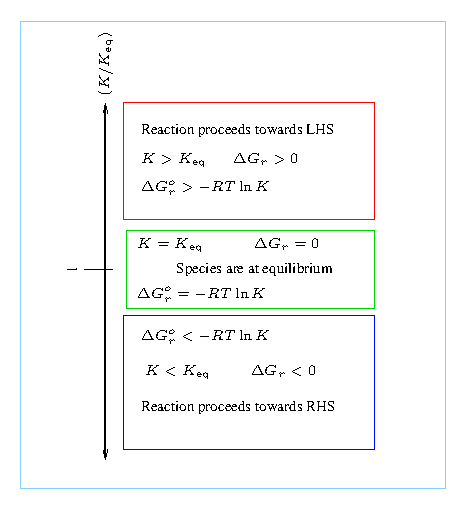
\includegraphics[scale=0.7]{images/c19-kchangefig.ps}
}
\end{center}
\caption{Schematic showing changes in reaction constant}
\label{kchange}
\end{figure}

\subsection{Entropy maximization method}

Using the definition of chemical potential as a form of work done by the system due to change in composition, we can write the following.

\begin{equation} dU = T \, dS - p \, dV + \sum_{i}{ \mu_i \, dn_i} \end{equation}

Rearranging the terms, we can write the entropy change for the system as:

\begin{equation} dS = \frac{dU}{T} + \frac{p \, dV}{T} - \frac{1}{T} \sum_{i}{ \mu_i \, dn_i} \end{equation}

We consider an isolated system consisting of $n_{\text{CO}_2}$, $n_\text{CO}$ and $n_{\text{O}_2}$ moles of the species $\text{CO}_2$, $\text{CO}$ and $\text{O}_2$, respectively.

The last term in the entropy expression is then elaborated as follows:
\begin{equation} \sum_{i}{ \mu_i \, dn_i} = \mu_{\text{CO}_2} \, dn_{\text{CO}_2}  +  \mu_\text{CO} \, dn_\text{CO}  + \mu_{\text{O}_2} \, dn_{\text{O}_2} \end{equation}

From the conservation of number of atoms of each element, we write the change in number of moles of species related as follows:

\begin{equation} 2 dn_{\text{O}_2} = -dn_\text{CO} - 2 dn_{\text{CO}_2} \end{equation}

\begin{equation} dn_\text{CO} = -dn_{\text{CO}_2} \end{equation}

We use these expressions to eliminate the variables $dn_\text{CO}$ and $dn_{\text{O}_2}$ from the above equation.

\begin{equation} \sum_{i}{ \mu_i \, dn_i} = \mu_{\text{CO}_2} \, dn_{\text{CO}_2}  +  \mu_\text{CO} \, \left( - dn_{\text{CO}_2} \right) + \frac{1}{2} \mu_{\text{O}_2} \, \left( -2dn_{\text{CO}_2} -dn_\text{CO} \right) \end{equation}

\begin{equation} \sum_{i}{ \mu_i \, dn_i} = \mu_{\text{CO}_2} \, dn_{\text{CO}_2}  +  \mu_\text{CO} \, \left( - dn_{\text{CO}_2} \right) + \frac{1}{2} \mu_{\text{O}_2} \, \left( -2dn_{\text{CO}_2} + dn_{\text{CO}_2} \right) \end{equation}

\begin{equation} \sum_{i}{ \mu_i \, dn_i} = \left( \mu_{\text{CO}_2} -  \mu_\text{CO} - \frac{1}{2} \mu_{\text{O}_2}  \right) \, dn_{\text{CO}_2} \end{equation}

\begin{equation} \sum_{i}{ \mu_i \, dn_i} = \frac{1}{2} \left( 2 \mu_{\text{CO}_2} -  2\mu_\text{CO} - \mu_{\text{O}_2}  \right) \, dn_{\text{CO}_2} \end{equation}

Substituting this into the expression for entropy change,

\begin{equation} dS = \frac{dU}{T} + \frac{p \, dV}{T} - \frac{1}{2T} \left( 2 \mu_{\text{CO}_2} -  2\mu_\text{CO} - \mu_{\text{O}_2}  \right) \, dn_{\text{CO}_2} \end{equation}

For an isolated system, the change in internal energy and volume are zero. Thus, we can see that entropy maximization with respect to composition is possible when ${\partial S}/{\partial n_{\text{CO}_2}} = 0$. Thus, the equilibrium - when entropy is maximum - is when the following condition is satisfied.

\begin{equation} 2 \mu_{\text{CO}_2} -  2\mu_\text{CO} - \mu_{\text{O}_2} = 0 \end{equation}

On the lines of earlier method, we define $\Delta G_r$ as follows:

\begin{equation} \Delta G_r \equiv 2 \mu_{\text{CO}_2} -  2\mu_\text{CO} - \mu_{\text{O}_2} \end{equation}


\begin{equation} dS = \frac{-\Delta G_r}{2T} \, dn_{\text{CO}_2} \end{equation}

When $\Delta G_r < 0$, the reaction should proceed in the direction dictated by a spontaneous increase in entropy. This is possible only when $dn_{\text{CO}_2}$ is positive. This implies that the number of moles of $\text{CO}_2$ must increase. Thus, the reaction proceeds towards RHS.

Similarly, when $\Delta G_r > 0$, the reaction should proceed in the direction dictated by a spontaneous increase in entropy. This is possible only when $dn_{\text{CO}_2}$ is negative. This implies that the number of moles of $\text{CO}_2$ must decrease. Thus, the reaction proceeds towards LHS.

The chemical potentials for each phase can now be expanded as $ \mu_i = \mu^o_i + RT \ln a_i$ to see the conclusions above extended to a variation in partial pressures of individual species.

\subsection{Ellingham Diagram}

If we would like to express the standard Gibbs energy for any reaction in terms of standard enthalpy and entropy of the reaction, we can say:

\begin{equation}
\Delta G^o (T) = \Delta H^o (T) - T \Delta S^o(T)
\end{equation}

The variation of enthalpy with temperature at a given pressure is given by:

\begin{equation}
\Delta H^o (T) = \Delta H^o (T_o) + \int_{T_o}^{T}{ \Delta C_p^o(T) dT}
\end{equation}

Where, $\Delta C_p^o$ is the heat capacity of the components on RHS minus the heat capacity of the components on the LHS, with the coefficients given as per the stoichiometric equation.

Similarly, we can write the variation of entropy with temperature at a given pressure as:

\begin{equation}
\Delta S^o (T) = \Delta S^o (T_o) + \int_{T_o}^{T}{\frac{\Delta C_p^o(T)}{T} dT}
\end{equation}

Compared to the heats of reactions (latent component, usually in hundreds of kilojoules), the heat exchanges for altering the temperatures of reactants or products (sensible component, usually in tens of kilojoules) are much smaller. Thus in both the above equations, the second term on RHS can be taken as negligible.

Thus, $\Delta G^o_r$ is expressed as simple linear relationship with temperature as $A + BT$. Here, $A \approx \Delta H^o (T_o) = \sum_\text{RHS}{n_i H_i}-\sum_\text{LHS}{n_i H_i}$. The constants $n_i$ are taken from the stoichiometric reaction. Similarly, $-B \approx \Delta S^o(T_o) = \sum_\text{RHS}{n_i S_i}-\sum_\text{LHS}{n_i S_i}$

The sign of $B$ is negative when the total entropy of the species on the RHS is more than that on the LHS. Remember that the molar entropy of a gaseous phase is always much higher that the corresponding condensed phases. So, we could say the following: If the reaction is written such that the number of moles of gaseous species on the LHS is more, then the constant $B$ is positive. This is the case for most of the oxidation reactions for metals. However, the case of $ 2 \text{C} + \text{O}_2 = 2 \text{CO}_2 $ will have negative value of $B$. 

The plot of $\Delta G^o (T)$ as a function of $T$ is known as Ellingham diagram.

\subsection{References}
\begin{enumerate}
\item Chapter 11 of {\em Thermodynamics in Materials Science} by Robert DeHoff, Second Edition, CRC Press (2006), ISBN: 9780849340659
\item Chapter 17 of {\em Materials Thermodynamics} by Y. Austin Chang and W. Alan Oates, Wiley (2010), ISBN: 9780470484142
\item Chapter 10 of {\em Materials Thermodynamics with emphasis on chemical approach} by Hae-Geon Lee, World Scientific Press (2012), ISBN:  9789814368056
\end{enumerate}

